\chapter{Testy oprogramowania}

Testowanie oprogramowania ma na celu weryfikację opracowanych rozwiązań. Odpowiednio przygotowane testy pozwalają na szybką detekcję błędu, a także rozwiązanie jego przyczyny. W zależności od przyjętej ideologi, testy oprogramowania przygotowywane są przed lub po opracowaniu właściwego kodu programu. Szczególnym przypadkiem testów pisanych po zakończeniu implementacji są testy pisane nigdy.\\

Metodyka realizacji testów jest dobrze rozwinięta dla typowych aplikacji webowych, co skutkuje dużym wyborem narzędzi umożliwiających testowanie i "mockowanie" modułów. W przypadku symulacji i gier komputerowych sytuacja jest odmienna. Oprócz sprawdzenia poprawności kodu niezbędna jest walidacja samego symulowanego modelu. Służą do tego specjalne mechanizmy, które wykształciły się w branży lotniczej.\\

Przygotowane testy można podzielić na cztery kategorie: testy jednostkowe, testy integracyjne, testy end-to-end oraz testy walidujące poprawność symulacji.

\section{Testy jednostkowe}

Testy jednostkowe to rodzaj testów oprogramowania, które sprawdzają indywidualne jednostki kodu, takie jak funkcje, metody czy klasy. Ich celem jest sprawdzenie, czy poszczególne fragmenty programu działają poprawnie, zgodnie z oczekiwaniami.
W programach zawierających elementy fizyki szczególnie ważne jest przetestowanie czy komponenty odpowiedzialne za przedstawienie poszczególnych zjawisk mają sens fizyczny.
W opracowanej symulacji kompleksowo przetestowane zostały obliczenia fizyczne, konwertery, klasa ODE, klasa Controller oraz model atmosfery ISA. 

\subsection{Testy klasy implementującej model atmosfery ISA}

Model wzorcowy atmosfery ISA (International Standard Atmosphere) to model matematyczny pozwalający na oszacowanie warunków atmosferycznych takich jak temperatura, ciśnienie oraz gęstość powietrza w zależności od wysokości nad poziomem morza. W bazowej formie pozwala na poprawne oszacowanie parametrów w warstwie przypowierzchniowej tj. troposferze. Testy klasy sprawdzają czy wartości obliczane przez klasę są zgodne z wartościami dostępnymi w tablicach. Analiza kilkunastu punktów testowych pozwala z dużym prawdopodobieństwem potwierdzić poprawność implementacji.

\subsection{Testy metod całkowania równań różniczkowych}

W klasie ODE znajduje się implementacja algorytmów całkowania równań różniczkowych. Główną funkcją w klasie jest funkcja \texttt{step(...)} wykonująca jeden krok całkowania. Testy dotyczące tej klasy pokrywają kwestie programowe takie jak poprawne tworzenie i dekonstrukcja klasy, ale także mają za zadanie sprawdzenie fizycznej poprawności tej klasy. W tym celu sprawdzone zostały następujące scenariusze:

\begin{enumerate}
\item funkcja prawych stron przyjmuje wartość stałą równą zeru. Sprawdzenie, czy całkowana zmienna nie ulega zmianie
\item funkcja prawych stron przyjmuje wartość stałą. Jako, że każda z metod całkowania powinna być co najmniej pierwszego rzędy, sprawdzane jest czy rozwiązanie jest zgodne z analitycznym.
\item sprawdzenie liczby wywołań funkcji prawych stron. Każda z metod deklaruje liczbę niezbędnych wywołań funkcji prawych stron. Jako, że wywołania mogą być potencjalnie kosztowne, sprawdzane jest czy liczba wywołań jest zgodna z deklarowaną, optymalną liczbą wywołań wynikającą z teorii.
\item całkowanie równań różniczkowych opisujących oscylator harmoniczny bez tłumienia (masa na sprężynie). W trakcie całkowania w każdym kroku obliczana jest całkowita energia mechaniczna, będąca sumą energii kinetycznej i energii potencjalnej sprężystości. Sprawdzane jest czy całkowita energia mieści się w żądanym polu tolerancji, symetrycznym względem energii początkowej układu.
\end{enumerate}
 
\subsection{Testy implementacji regulatorów}

Interfejs Controller definiuje klasy reprezentujące różne regulatory wykorzystywane przez układ sterowania. Główną funkcją w interfejsie jest funkcja \texttt{calc(...)} obliczająca wyjście z regulatora dla przekazanej wartości zadanej i mierzonej zmiennej regulowanej. Do testów przygotowane zostały obiekty regulatorów z doświadczalnie dobranymi nastawami. Testy tej klasy mają na celu potwierdzić poprawność regulacji poprzez realizację następujących scenariuszy:

\begin{enumerate}
\item sprawdzenie, czy znak wyjścia z regulatora jest zgodny ze znakiem uchybu tj. różnicy pomiędzy wartością zadaną a wartością aktualną.
\item symulacja regulacji w układzie o jednym stopniu swobody, w którym wartość wyjściowa z regulatora wpływa na pochodną ze zmiennej regulowanej. Scenariusz reprezentuje uproszczony model regulacji temperatury w pomieszczeniu, z którego ucieka ciepło, a regulator steruje grzejnikiem dostarczającym ciepło. Badane jest czy po odpowiednim czasie ustalenia temperatura w pomieszczeniu utrzymuje się w założonym polu tolerancji. Dodatkowo w trakcie testu logowane są przebiegi wartości regulowanej. Ma to na celu umożliwić organoleptyczną analizę poprawności działania regulatora. Przykładowe przebiegi ilustruje rysunek (\ref{controller_plot}).
\end{enumerate}

\begin{figure}[!th]
	\centering
	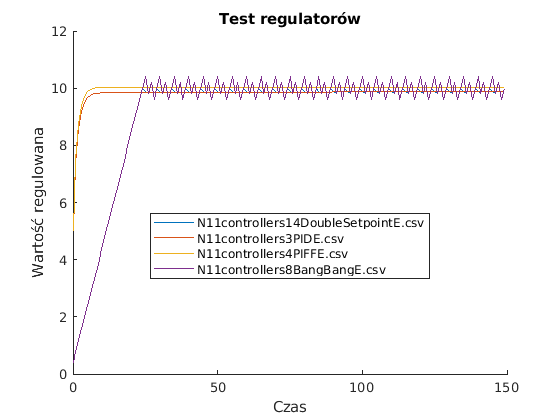
\includegraphics[width=0.7\textwidth]{controller_plot.png}
	\caption{Przebieg testu regulatorów}
	\label{controller_plot}
\end{figure}
\newpage

\section{Testy integracyjny}

Testy integracyjne są kolejnym etapem testowania oprogramowania, który koncentruje się na weryfikacji poprawności całościowego działania modułów systemu. Ich celem jest sprawdzenie, czy poszczególne części oprogramowania będą działać w połączeniu ze sobą. Polegają one najczęściej na uruchomieniu wybranego modułu w izolacji i sztucznym wygenerowaniu zapytań i odpowiedzi pochodzących z innych modułów. Rozbudowane testy integracyjne zostały napisane dla modułów UAV\_drop\_physic oraz UAV\_visualization. Fizyka obiektów jest testowana pod względem tworzenia nowych obiektów oraz ich reakcji na fizyczne bodźce. Testowanie wizualizacji przeprowadzone jest za pomocą skryptu w języku Python, który imitując serwer inicjalizuje wizualizację oraz wysyła dane, które tester jest w stanie zweryfikować na podstawie wygenerowanego obrazu.

\subsection{Testy modułu UAV\_drop\_physic}

Moduł \textbf{UAV\_drop\_physic} odpowiada za symulację lotu pocisków i ładunków, a wiec obiektów nie posiadających własnego źródła napędu. Testy modułu zawierają sprawdzenie poprawności uruchomienia i zamknięcia modułu, nawiązanie z nim komunikację, ale także sprawdzają poprawność działania przez symulację następujących scenariuszy testowych:

\begin{enumerate}
\item sprawdzenie mechanizmu dodawania i usuwania obiektów z symulacji. Sprawdzana jest poprawność nadawania identyfikatorów kolejnym obiektom,
\item symulacja spadku swobodnego bez oporu powietrza. Sprawdzane jest czy zmianie ulega jedynie składowa pionowa prędkości i położenia oraz czy wynik symulacji jest zgodny z rozwiązaniem analitycznym z przyjętą tolerancją.
\item symulacja spadku swobodnego z silnym oporem powietrza (spadochroniarz). Podobnie jak w powyższym teście sprawdzane jest osiągniecie określonej prędkości i położenia po zakładanym czasie.
\item symulacja wpływu siły zewnętrznej. Do spadającego swobodnie obiektu przyłożona zostaje pozioma siła. Sprawdzane jest czy horyzontalne składowe położenia odpowiadają rozwiązaniu analitycznemu dla ruchu przyspieszonego.
\item symulacja odbić od płaszczyzn, wykorzystywana w mechanizmie kolizji. Sprawdzane są odbicie plastyczne, sprężyste i sprężyste z tarciem. W każdym z testów sprawdzane są cechy charakterystyczne położenia i prędkości po odbiciu.
\item symulacja długotrwałego lotu w silnym wietrze. Dla obiektu na który działa silny wiatr poziomy oczekiwane jest, że po dostatecznie długim czasie osiągnie on prędkość zgodną z działającym wiatrem. 
\end{enumerate}
\subsection{Testy integracyjne wizualizacji}

Test integracyjny wizualizacji uruchomić można za pomocą skryptu \\ \texttt{visualization\_tests.py}, gdzie argumentami jest ścieżka do pliku wykonywalnego Javy, za pomocą której powinien zostać uruchomiony klient, katalog, w którym znajduje się klient, nazwa archiwum JAR klienta oraz suma kontrolna assetów, które wizualizacja ma wykorzystać. \\


Test rozpoczyna się od utworzenia wszystkich wymaganych gniazd sieciowych (socket'ów) obsługiwanych przez serwer. Następnie do katalogu klienta przekopiowywane są dane testowe w postaci konfiguracji aplikacji, przypisań kontrolera oraz parametrów drona i uruchamiana jest aplikacja. Skrypt następnie nawiązuje połączenie z aplikacją i testuje proces rozpoczęcia symulacji od pobrania przez klienta danych o serwerze, wysłaniu przez klienta odpowiednich parametrów BSP po jego prośbę o utworzenie statku. Po poprawnej wymianie informacji z aplikacją zmiany wprowadzone przez dane testowe są wycofane. Następnie skrypt przechodzi do wysyłania co 5ms wygenerowanego stanu BSP, który jest widoczny z poziomu ekranu wizualizacji. Rutyna obejmuje poruszanie się oraz obrotu statku we wszystkich osiach oraz fluktuację prędkości obrotowej każdego z silników.  

\section{Testy End-to-end}

Testy end-to-end (E2E) są rodzajem testów oprogramowania, które sprawdzają poprawność działania systemu jako całości, od rozpoczęcia działania aż do oczekiwanych wyników. W ramach testów end-to-end przetestowane zostało działanie serwera, który rozpoczyna swoje wywołanie od modułu UAV\_aggregator. Uruchamia on moduły symulacji fizyki i kontrolera, sprawdzając, czy zainicjalizowały się poprawnie. 
Następnie generowana jest komunikacja z wizualizacją, symulująca wejście od użytkownika. Pozwala ona na przetestowanie reakcji systemu na przychodzące wiadomości.
Ostatecznie serwer wyłącza moduły i weryfikuje poprawne zatrzymanie wszystkich procesów. 

\section{Testy walidujące}

Testy walidacyjne moją na celu potwierdzić użyteczność symulacji. To na podstawie ich wyniku podjęta zostaje decyzja, czy wyniki symulacji są wiarygodne i mogą zostać wykorzystane w analizach. W praktyce przygotowywania symulatorów lotniczych walidacja stanowi ostatni etap metody 4M, której poszczególnymi etapami są:
\begin{itemize}[noitemsep]
\item Manoeuvre -- zaplanowanie i wykonanie eksperymentu
\item Measurement -- pomiar i rejestracja stanu statku powietrznego
\item Method -- dobór odpowiedniej metody identyfikacji i estymacja
\item Model -- symulacja przygotowanego modelu matematycznego
\item Walidacja modelu -- sprawdzenie poprawności przygotowanego modelu
\end{itemize}

Jedną z najpopularniejszych metod walidacji są analiza sensu fizycznego modelu oraz tzw. dowód zgodności. Analiza sensu fizycznego modelu polega na sprawdzeniu, czy zachowanie symulowanego modelu w określonych scenariuszach odpowiada przewidywanym odpowiedziom. Do podstawowych badań należy sprawdzenie poprawności zachowania w reakcji na wychylenia powierzchni sterowych i położenia przepustnicy. Dodatkowa analiza kąta natarcia i ślizgu pozwala na porównanie wartości symulowanych z testami tunelowymi. Powyższe testy mają charakter lokalny, badający pewien podzbiór stanów BSP. W przeciwieństwie do tego na podjęcie całkowitego werdyktu pozwala dowód zgodności. Polega on na pełnym zarejestrowaniu stanu obiektu w locie i symulacji oraz sprawdzenie, czy są one ze sobą zgodne z określoną tolerancją. Tolerancja ta może wynikać ze skończonej dokładności czujników pomiarowych, szumu przetwarzania lub tolerancji Maximum Unnoticeable Added Dynamics, czyli największego dopuszczalnego błędu, który pozostanie niezauważony przez doświadczonego użytkownika. Ostatni z parametrów jest szczególnie użyteczny w przypadku symulatorów do szkolenia pilotów.\\

Ze względu na charakter pracy, budowa symulacji w oparciu o badanie konkretnego modelu nie jest możliwa. Przyjęty model stanowi fuzję cech modeli pojawiających się w literaturze, dla których nie wszystkie współczynniki są jasno określone. Zatem z pominięciem powyższych etapów przygotowana symulacja nie odwzorowuje wiernie konkretnego statku. Nie zmienia to faktu, że uniwersalny model również może być weryfikowany, ze względu na zachowania, które powinny wystąpić zawsze, niezależnie od konfiguracji. W ten sposób można zaplanować zbiór testów manualnych, które pozwalają szybko potwierdzić poprawność modelu. Przykładowe zachowania, które podlegają sprawdzeniu to:
\begin{itemize}[noitemsep]
\item BSP poprawnie odpowiada na wychylenia osi joysticka, przynajmniej co do kierunku obrotu.
\item BSP posiada cechy bryły sztywnej poruszającej się w powietrzu.
\item W przypadku statków stabilnych aerodynamicznie, BSP pozostaje stabilny w trakcie lotu: BSP sam minimalizuje ślizg, gasi prędkości kątowe lub je ogranicza.
\item W przypadku wielowirnikowców poprawnie realizowany jest zawis
\item W przypadku płatowców, do utrzymania wysokości przy prędkości przelotowej potrzebny jest dodatni kąt natarcia. W locie odwróconym wymagany kąt natarcia jest większy.
\end{itemize}